\apendice{Documentación técnica de programación}

\section{Introducción}
En este anexo se muestra toda la información necesaria para que un desarrollador pueda poner en funcionamiento el \textit{software} de este proyecto.
Además, se da una explicación sobre la estructura del código y aquellos aspectos que puedan ser importantes para cualquier desarrollador que vea por primera vez el código desarrollado.

\section{Estructura de directorios}
La estructura de los directorios del proyecto es la siguiente:
\begin{itemize}
\item \textbf{docs:} Contiene la documentación del proyecto.
\item \textbf{src:} Dentro de este directorio se encuentra el código fuente del proyecto desarrollado.
\end{itemize}

Este anexo va a centrarse en la explicación del contenido del directorio \texttt{src}.
En la figura~\ref{fig:directorios} se puede ver la distribución de los directorios que se encuentran dentro de \texttt{src}.

\begin{figure}
	\centering
	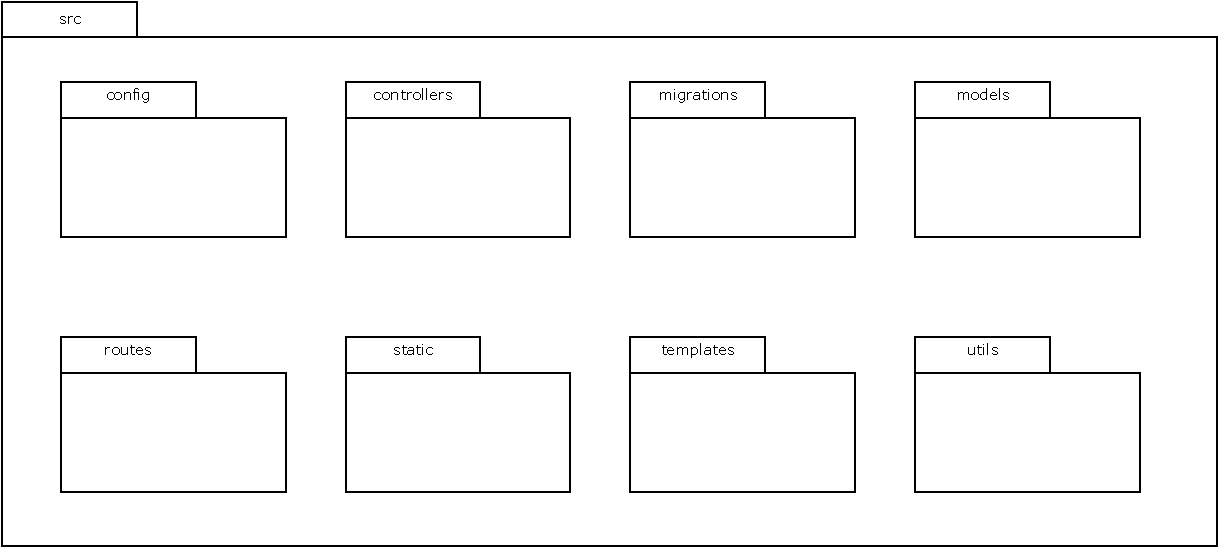
\includegraphics[width=\textwidth]{../img/Anexos/directorios.pdf}
	\caption{Directorios del proyecto}\label{fig:directorios}
\end{figure}

A continuación se da una explicación de lo contenido en cada directorio:
\begin{itemize}
\item \texttt{src:} 
Es el directorio principal del código fuente del proyecto que contiene a todos los demás. 
Además, en su interior se encuentra el fichero \texttt{app.py} desde el que se carga la configuración y se arranca la aplicación, el fichero \texttt{forms.py} que contiene todos los formularios generados a partir de al biblioteca WTForms y el fichero \texttt{decorators.py} que contiene aquellas funciones encargadas de detectar los permisos del usuario activo y su \textit{token}.
Por otro lado, también se encuentran los ficheros \texttt{Procfile} necesario para desplegar la aplicación en Heroku, \texttt{requirements.txt} que contiene todas las bibliotecas junto a su versión requerida y el fichero \texttt{runtime.txt} también necesario para desplegar en Heroku donde se indica la versión de Python.

\item \texttt{config:} 
Contiene tres ficheros necesarios para la configuración del proyecto.
El fichero \texttt{config.py} indica la configuración general del proyecto mientras que los ficheros \texttt{development.py} y \texttt{production.py} contienen la configuración necesaria para el despliegue en modo desarrollo y modo producción respectivamente.

\item \texttt{controllers:}
En este directorio se encuentran todos los controladores del proyecto.

\item \texttt{migrations:}
Es un directorio perteneciente a la librería Flask-Migrate. 
Este directorio es utilizado para almacenar la configuración de la biblioteca y las diferentes migraciones creadas para actualizar la base de datos evitando la pérdida de información almacenada. (En principio, no sería necesario modificar nada de este directorio).

\item \texttt{models:}
Aquí se encuentran todos los ficheros respectivos a los modelos de la aplicación web. Es decir, aquellos objetos que se crean y almacenan en la aplicación.
Desde cada uno de estos ficheros también se define la estructura de sus tablas en la base de datos.

\item \texttt{routes:}
Este directorio almacena los diferentes ficheros que definen las rutas de la aplicación, organizadas por \textit{blueprints}.

En estos ficheros se indican los decoradores de cada ruta y la acción del controlador asociada que se debe ejecutar con la petición a esa ruta. 
Además, se define el tipo de petición HTTP permitida por ruta.

\item \texttt{static:} 
Como su nombre indica, este directorio contiene todos aquellos ficheros estáticos de la aplicación que van a ser cargados por las vistas. 
Los ficheros que contiene son accesibles desde un navegador y aquí se almacenan imágenes, ficheros CSS, ficheros de JavaScript y las librerías de JavaScript cargadas desde el sistema de gestión de paquetes NPM, junto al fichero de configuración donde se indican las bibliotecas y su versión llamado \texttt{package.json}.

\item \texttt{templates:}
Este directorio agrupa todas aquellas vistas de la aplicación web.
Dentro se encuentra dividido a su vez por otros directorios con el nombre de los diferentes modelos para tener más organizadas las vistas.

En este directorio también se encuentra el fichero \texttt{base\_template.html} que define la plantilla base de todas las demás vistas.
Desde este fichero se define la carga de los ficheros CSS y \textit{scripts} de JavaScript, además de otros elementos como el menú de la aplicación.

En este fichero todos los elementos se encuentran divididos por bloques para cargar solo aquellos necesarios.
Por ejemplo, el footer solo se carga en la vista de \textit{login}, pero el bloque de carga se define aquí.

\item \texttt{utils:}
Este directorio está creado para mejorar la carga y organización de la aplicación.
Dentro del directorio se encuentra el fichero \texttt{db.py} donde se cargan las bibliotecas relativas a la base de datos como SQLAlchemy o Flask-Migrate.
\end{itemize}

\section{Manual del programador}
En esta sección se van exponer algunos detalles necesarios para el entendimiento del código desarrollado teniendo en cuenta la explicación de la estructura de directorios dada en la sección anterior.

Como se ha comentado antes, los archivos necesarios para la configuración del proyecto se encuentran dentro del directorio \texttt{config}.

El fichero \texttt{config.py} contiene la configuración general del proyecto. En la la figura~\ref{fig:ficheroConfig} se muestra el contenido del fichero. En él se puede ver como se indica la clave secreta junto a otras configuraciones como el modo \textit{debug}, las sesiones, el \textit{email} del administrador, etc.

\begin{figure}
	\centering
	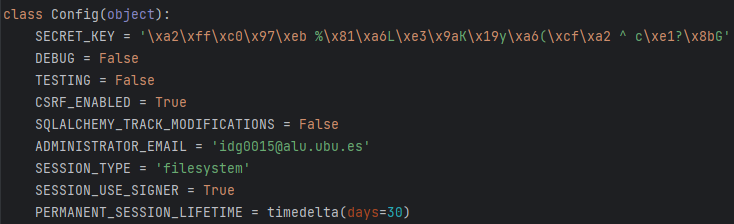
\includegraphics[width=\textwidth]{../img/Anexos/ManualProgramador/config.png}
	\caption{Fichero config.py}\label{fig:ficheroConfig}
\end{figure}

En la figura~\ref{fig:ficheroDev} se puede ver el fichero \texttt{development.py}. 
En este fichero se activa el modo \textit{debug} y se indica cual va a ser la base de datos. 
La configuración de este fichero sólo se cargará si en el sistema se encuentra la variable de entorno \texttt{FLASK\_ENV}. 
Esta carga se puede ver en el fichero \texttt{app.py}. 
Por defecto se utiliza el valor \texttt{development}, por lo que si la variable no está definida se tomará la configuración de desarrollo.

\begin{figure}
	\centering
	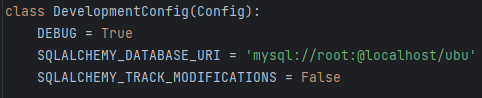
\includegraphics[width=\textwidth]{../img/Anexos/ManualProgramador/development.png}
	\caption{Fichero development.py}\label{fig:ficheroDev}
\end{figure}

Por último, en la figura~\ref{fig:ficheroProd} se muestra la configuración del proyecto para el caso de tener el entorno definido como producción.

En este caso la ruta de la base de datos se obtiene desde una variable de entorno llamada \texttt{JAWSDB\_MARIA\_URL} que debe encontrarse definida en el sistema.

Este nombre puede cambiarse sin problema, pero se le dio este nombre debido a que en Heroku, plataforma donde se ha desplegado la aplicación, tiene ese nombre la variable.

\begin{figure}
	\centering
	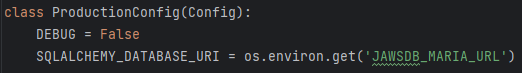
\includegraphics[width=\textwidth]{../img/Anexos/ManualProgramador/production.png}
	\caption{Fichero production.py}\label{fig:ficheroProd}
\end{figure}


\section{Compilación, instalación y ejecución del proyecto}
En esta sección se van a especificar los pasos que se deben seguir para poder desplegar la aplicación de forma correcta para poder ser utilizada.

Lo primero y más importante es conseguir el código fuente. 
Este se puede descargar desde el repositorio\footnote{\url{https://github.com/idg0015/Aplicacion-de-gestion-del-PDI-de-un-area-de-la-UBU}} del proyecto.

Para realizar la descarga se puede utilizar la opción de GitHub de descargar desde la página web mediante un archivo ZIP o utilizar Git para realizar una clonación del repositorio mediante el comando \texttt{git clone}.

\subsection{Preparación del entorno}
Para el desarrollo de la aplicación se ha utilizado el IDE PyCharm y se recomienda su uso ya que aligera el proceso de preparación del entorno al contener perfiles ya pre-creados para distintos \textit{frameworks} siendo uno de ellos Flask.

De todas forma, en caso contrario, para preparar el entorno de trabajo lo primero que se debe instalar en el sistema es Python.
Esto se puede realizar mediante una descarga de su web\footnote{Se puede descargar desde aquí: \url{https://www.python.org/downloads/}} y seguir los pasos del instalador. Para este proyecto se ha utilizado Python 3.9.

También se debe instalar algún sistema gestor de bases de datos como MariaDB o MySQL.

Con Python instalado, lo recomendable es crear un entorno virtual para ejecutar Python, de esta manera se pueden tener diferentes versiones de Python instaladas y, según el entorno, ejecutar una u otra.
Para ello, se debe ejecutar el comando \texttt{virtualenv env} para crear el entorno y acto seguido ejecutar \texttt{env\textbackslash{}Scripts\textbackslash{}activate.bat} (en el caso de Windows) para indicar que queremos utilizar el entorno.
Esto hará que en el \textit{prompt} de la consola aparezca la palabra <<(env)>>, lo que nos asegurará de que estamos trabajando bajo el entorno.

Por último, en la raíz del proyecto se debe ejecutar el comando \texttt{pip install -r requirements.txt}.
De esta forma quedarán instaladas las bibliotecas necesarias para Python.

Para instalar las bibliotecas de JavaScript necesarias para el uso de la aplicación se debe ejecutar el comando \texttt{npm i} a nivel de carpeta \texttt{src/static}, donde se encuentra el archivo <<package.json>> en el que se indican las bibliotecas a descargar junto a su versión. 

Con todo esto realizado ya tendríamos configurado lo necesario para poder arrancar la aplicación.
Para ello se deben seguir los siguientes pasos:
\begin{enumerate}
\item Ejecutar el comando \texttt{export FLASK\_APP=app.py} para exportar la variable de entorno que indica el fichero desde el que arranca la aplicación.
\item Se podría hacer lo mismo para FLASK\_ENV y FLASK\_DEBUG con los valores <<development>> y <<1>> respectivamente para su uso en desarrollo, pero no debería ser algo necesario ya que esto se encuentra en los ficheros de configuración de la aplicación.
\item Ejecutar el comando \texttt{python -m flask run}.
\end{enumerate}

Con esto realizado la aplicación habría arrancado y al acceder a la dirección <<127.0.0.1:5000>> debería verse la aplicación.
En este paso lo único que necesario para poder acceder al contenido de la aplicación es almacenar un docente en la base de datos desde el sistema gestor utilizado que tenga como correo electrónico el mismo utilizado para iniciar sesión en el Moodle de una universidad.

\subsection{Despliegue en Heroku}
En este apartado se va a dar la explicación para desplegar la aplicación web en la plataforma Heroku.

En primer lugar es necesario tener los ficheros <<requirements.txt>>, <<runtime.txt>>, <<Procfile>> y <<package.json>> a nivel de la raíz del directorio a subir, ya que si no Heroku no será capaz de poder utilizarlos (estos archivos ya se encuentran incluidos en el repositorio).

Es importante saber que el fichero <<package.json>> no debe ser el mismo que se encuentra en el directorio <<static>>, donde se indican los paquetes a instalar, si no que debe ser un fichero que apunte a este otro, desde donde sí se hará la instalación. 
Esto es debido a que Heroku no es capaz de detectar el archivo <<package.json>> si se encuentra dentro del directorio <<static>>. Además, si ponemos el fichero tal cual, los paquetes se instalaran en la raíz del proyecto y no en la carpeta static.

El contenido del fichero <<package.json>> en la raíz del proyecto debería ser algo parecido a lo mostrado en la figura~\ref{fig:ficheroPackage}.

Como se puede ver, cuenta con una instrucción <<\textit{postinstall}>> donde se indica que se mueva al directorio <<static>> y ahí haga la instalación de paquetes.
Cuando se haga el \texttt{npm install} consultará el fichero <<package.json>> de la carpeta <<static>>.

\begin{figure}
	\centering
	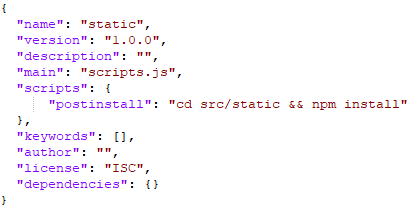
\includegraphics[width=.8\textwidth]{../img/Anexos/ManualProgramador/package.png}
	\caption{Fichero package.json de la raíz del proyecto}\label{fig:ficheroPackage}
\end{figure}


\section{Pruebas del sistema}
En esta sección se van a realizar distintas pruebas para asegurar que el \textit{software} desarrollado funciona de la forma esperada y para corregir los fallos en caso contrario.

\subsection{Casos de prueba}
A continuación se presentan todos los casos de prueba realizados.

\begin{table}[H]
\small
\begin{tabular}{p{.17\textwidth} p{.12\textwidth} p{.2\textwidth} p{.2\textwidth} p{.14\textwidth}}
\cellcolor{gray!25}
ID   & CP1 & \cellcolor{gray!25} Prioridad   & Alta \\ \hline
\cellcolor{gray!25} Fecha	&	\multicolumn{4}{l}{26/06/2023} \\ \hline
\cellcolor{gray!25} Descripción		&	\multicolumn{4}{l}{Probar el inicio de sesión correcto de la aplicación} \\ \hline                                            
\cellcolor{gray!25}
Precondición  & \multicolumn{4}{l}{No tener sesión iniciada} \\ \hline
\cellcolor{gray!25} Postcondición & \multicolumn{4}{l}{No hay sesión iniciada}                                                                                                      \\ \hline
\rowcolor{gray!25}
\textbf{Paso}   & \textbf{Entrada} & \textbf{Salida esperada} & \textbf{Salida real} & \textbf{Resultado} \\ \hline
Acceder a la página de \textit{login} 
& \texttt{/login}                                                                             
& Redirección a la página de \textit{login}                                    
& Redirección a la página de \textit{login}                                   
& Correcto                            
\\ \hline
Rellenar formulario de inicio de sesión
& Email: idg0015-
@alu.ubu.-
es, Contraseña: XXXX                                                                                                        
& Datos introducidos                               
& Datos introducidos                                
& Correcto                            
\\ \hline
Iniciar sesión
& Hacer clic en <<Iniciar sesión>>
& Redirección a la página principal                                 
& Redirección a la página principal                                 
& Correcto                            
\\ \hline                 
\end{tabular}
\caption{Caso de prueba 1: Inicio de sesión correcto.}
\end{table}

\begin{table}[H]
\small
\begin{tabular}{p{.17\textwidth} p{.12\textwidth} p{.2\textwidth} p{.2\textwidth} p{.14\textwidth}}
\cellcolor{gray!25}
ID   & CP2 & \cellcolor{gray!25} Prioridad   & Alta \\ \hline
\cellcolor{gray!25} Fecha	&	\multicolumn{4}{l}{26/06/2023} \\ \hline
\cellcolor{gray!25} Descripción		&	\multicolumn{4}{l}{Probar el inicio de sesión fallido de la aplicación} \\ \hline                                            
\cellcolor{gray!25}
Precondición  & \multicolumn{4}{l}{No tener sesión iniciada} \\ \hline
\cellcolor{gray!25} Postcondición & \multicolumn{4}{l}{No hay sesión iniciada}                                                    \\ \hline
\rowcolor{gray!25}
\textbf{Paso}   & \textbf{Entrada} & \textbf{Salida esperada} & \textbf{Salida real} & \textbf{Resultado} \\ \hline
Acceder a la página de \textit{login} 
& \texttt{/login}                                                                             
& Redirección a la página de \textit{login}                                    
& Redirección a la página de \textit{login}                                   
& Correcto                            
\\ \hline
Rellenar formulario de inicio de sesión
& Email: test@-
gmail.com, Contraseña: 1234
& Datos introducidos                               
& Datos introducidos                               
& Correcto                            
\\ \hline
Iniciar sesión
& Hacer clic en <<Iniciar sesión>>
& Mensaje: ``Usuario o contraseña incorrectos''
& Mensaje: ``Usuario o contraseña incorrectos''
& Correcto                            
\\ \hline                 
\end{tabular}
\caption{Caso de prueba 2: Inicio de sesión fallido.}
\end{table}

\begin{table}[H]
\small
\begin{tabular}{p{.17\textwidth} p{.12\textwidth} p{.2\textwidth} p{.2\textwidth} p{.14\textwidth}}
\cellcolor{gray!25}
ID   & CP3 & \cellcolor{gray!25} Prioridad   & Alta \\ \hline
\cellcolor{gray!25} Fecha	&	\multicolumn{4}{l}{26/06/2023} \\ \hline
\cellcolor{gray!25} Descripción		&	\multicolumn{4}{l}{Probar la correcta creación de un centro} \\ \hline                                            
\cellcolor{gray!25}
Precondición  & \multicolumn{4}{l}{Tener sesión iniciada con permisos de modificación} \\ \hline
\cellcolor{gray!25} Postcondición & \multicolumn{4}{l}{No hay sesión iniciada}                                                    \\ \hline
\rowcolor{gray!25}
\textbf{Paso}   & \textbf{Entrada} & \textbf{Salida esperada} & \textbf{Salida real} & \textbf{Resultado} \\ \hline
Acceder a la página de centros 
& \texttt{/centros}                                                                             
& Redirección a la página de centros                                   
& Redirección a la página de centros                                   
& Correcto                            
\\ \hline
Abrir formulario de ingreso
& Clic en <<Nuevo>>
& Redirección a \texttt{/centros/nuevo}                               
& Redirección a \texttt{/centros/nuevo}                              
& Correcto                            
\\ \hline
Rellenar formulario de ata de centro
& Código interno: 13, Nombre: Escuela Politécnica Superior, Río Vena, Abreviatura: EPSv, Email del administrativo: departamentos.eps@ubu.es
& Datos introducidos                               
& Datos introducidos                               
& Correcto                            
\\ \hline
Crear centro
& Hacer clic en <<Añadir>>
& Mensaje: ``Centro añadido correctamente''. Redirección a \texttt{/centros}
& Mensaje: ``Centro añadido correctamente''. Redirección a \texttt{/centros}
& Correcto                            
\\ \hline                 
\end{tabular}
\caption{Caso de prueba 3: Creación correcta de centro.}
\end{table}

\begin{table}[H]
\small
\begin{tabular}{p{.17\textwidth} p{.13\textwidth} p{.2\textwidth} p{.2\textwidth} p{.13\textwidth}}
\cellcolor{gray!25}
ID   & CP4 & \cellcolor{gray!25} Prioridad   & Media \\ \hline
\cellcolor{gray!25} Fecha	&	\multicolumn{4}{l}{26/06/2023} \\ \hline
\cellcolor{gray!25} Descripción		&	\multicolumn{4}{l}{Creación de un centro faltando campos obligatorios} \\ \hline                                            
\cellcolor{gray!25}
Precondición  & \multicolumn{4}{l}{Tener sesión iniciada con permisos de modificación} \\ \hline
\cellcolor{gray!25} Postcondición & \multicolumn{4}{l}{No hay sesión iniciada}                                                    \\ \hline
\rowcolor{gray!25}
\textbf{Paso}   & \textbf{Entrada} & \textbf{Salida esperada} & \textbf{Salida real} & \textbf{Resultado} \\ \hline
Acceder a la página de centros 
& \texttt{/centros}                                                                             
& Redirección a la página de centros                                   
& Redirección a la página de centros                                   
& Correcto                            
\\ \hline
Abrir formulario de ingreso
& Clic en <<Nuevo>>
& Redirección a \texttt{/centros/nuevo}                               
& Redirección a \texttt{/centros/nuevo}                              
& Correcto                            
\\ \hline
Rellenar formulario de ata de centro
& Código interno: 13, Abreviatura: EPSv, Email del administrativo: departamentos.eps@ubu.es
& Datos introducidos                               
& Datos introducidos                               
& Correcto                            
\\ \hline
Crear centro
& Hacer clic en <<Añadir>>
& Mensaje: ``El nombre es obligatorio''
& Mensaje: ``El nombre es obligatorio''
& Correcto                            
\\ \hline                 
\end{tabular}
\caption{Caso de prueba 4: Creación de un centro faltando campos obligatorios.}
\end{table}

\begin{table}[H]
\small
\begin{tabular}{p{.17\textwidth} p{.12\textwidth} p{.2\textwidth} p{.2\textwidth} p{.14\textwidth}}
\cellcolor{gray!25}
ID   & CP5 & \cellcolor{gray!25} Prioridad   & Media \\ \hline
\cellcolor{gray!25} Fecha	&	\multicolumn{4}{l}{26/06/2023} \\ \hline
\cellcolor{gray!25} Descripción		&	\multicolumn{4}{l}{Eliminación de un centro sin titulaciones vinculadas} \\ \hline                                            
\cellcolor{gray!25}
Precondición  & \multicolumn{4}{p{.66\textwidth}}{Tener sesión iniciada con permisos de modificación y tener un centro creado sin titulaciones vinculadas} \\ \hline
\cellcolor{gray!25} Postcondición & \multicolumn{4}{l}{No hay sesión iniciada}                                                    \\ \hline
\rowcolor{gray!25}
\textbf{Paso}   & \textbf{Entrada} & \textbf{Salida esperada} & \textbf{Salida real} & \textbf{Resultado} \\ \hline
Acceder a la página de centros 
& \texttt{/centros}                                                                             
& Redirección a la página de centros                                   
& Redirección a la página de centros                                   
& Correcto                            
\\ \hline
Eliminar un centro
& Clic en icono de papelera de un centro de la tabla
& Alerta: ``¿Está seguro de eliminar el centro? No se podrá eliminar si tiene alguna titulación vinculada''
& Alerta: ``¿Está seguro de eliminar el centro? No se podrá eliminar si tiene alguna titulación vinculada''                              
& Correcto
\\ \hline
Aceptar la alerta
& Clic en <<Aceptar>>
& Mensaje: ``Centro eliminado correctamente''                              
& Mensaje: ``Centro eliminado correctamente''                             
& Correcto                            
\\ \hline                
\end{tabular}
\caption{Caso de prueba 5: Eliminación de un centro sin titulaciones vinculadas.}
\end{table}

\begin{table}[H]
\small
\begin{tabular}{p{.17\textwidth} p{.12\textwidth} p{.2\textwidth} p{.2\textwidth} p{.14\textwidth}}
\cellcolor{gray!25}
ID   & CP6 & \cellcolor{gray!25} Prioridad   & Alta \\ \hline
\cellcolor{gray!25} Fecha	&	\multicolumn{4}{l}{26/06/2023} \\ \hline
\cellcolor{gray!25} Descripción		&	\multicolumn{4}{l}{Eliminación de un centro con titulaciones vinculadas} \\ \hline                                            
\cellcolor{gray!25}
Precondición  & \multicolumn{4}{p{.66\textwidth}}{Tener sesión iniciada con permisos de modificación y tener un centro creado con titulaciones vinculadas} \\ \hline
\cellcolor{gray!25} Postcondición & \multicolumn{4}{l}{No hay sesión iniciada}                                                    \\ \hline
\rowcolor{gray!25}
\textbf{Paso}   & \textbf{Entrada} & \textbf{Salida esperada} & \textbf{Salida real} & \textbf{Resultado} \\ \hline
Acceder a la página de centros 
& \texttt{/centros}                                                                             
& Redirección a la página de centros                                   
& Redirección a la página de centros                                   
& Correcto                            
\\ \hline
Eliminar un centro
& Clic en icono de papelera de un centro de la tabla
& Alerta: ``¿Está seguro de eliminar el centro? No se podrá eliminar si tiene alguna titulación vinculada''
& Alerta: ``¿Está seguro de eliminar el centro? No se podrá eliminar si tiene alguna titulación vinculada''                              
& Correcto
\\ \hline
Aceptar la alerta
& Clic en <<Aceptar>>
& Mensaje: ``No se puede eliminar el centro porque tiene titulaciones asociadas''                              
& Mensaje: ``No se puede eliminar el centro porque tiene titulaciones asociadas''                             
& Correcto                            
\\ \hline                
\end{tabular}
\caption{Caso de prueba 6: Eliminación de un centro con titulaciones vinculadas.}
\end{table}

\begin{table}[H]
\small
\begin{tabular}{p{.17\textwidth} p{.12\textwidth} p{.2\textwidth} p{.2\textwidth} p{.14\textwidth}}
\cellcolor{gray!25}
ID   & CP7 & \cellcolor{gray!25} Prioridad   & Alta \\ \hline
\cellcolor{gray!25} Fecha	&	\multicolumn{4}{l}{26/06/2023} \\ \hline
\cellcolor{gray!25} Descripción		&	\multicolumn{4}{l}{Creación de una titulación} \\ \hline                                            
\cellcolor{gray!25}
Precondición  & \multicolumn{4}{p{.66\textwidth}}{Tener sesión iniciada con permisos de modificación y tener un centro creado} \\ \hline
\cellcolor{gray!25} Postcondición & \multicolumn{4}{l}{No hay sesión iniciada}                                                    \\ \hline
\rowcolor{gray!25}
\textbf{Paso}   & \textbf{Entrada} & \textbf{Salida esperada} & \textbf{Salida real} & \textbf{Resultado} \\ \hline
Acceder a la página de centros 
& /titulacio-
nes                                                                           
& Redirección a la página de titulaciones                                   
& Redirección a la página de titulaciones                                   
& Correcto                            
\\ \hline
Abrir formulario
& Clic en <<Nuevo>>
& Redirección a /titulaciones/nuevo
& Redirección a /titulaciones/nuevo
& Correcto
\\ \hline
Rellenar formulario
& Código interno: 63, Nombre: Gº en Ing, Informática, Abreviatura: GºII, URL: https://www.ubu.es/grado-en-ingenieria-informatica, Centro: Escuela Politécnica Superior, Río Vena
& Datos introducidos                            
& Datos introducidos
& Correcto                            
\\ \hline   
Crear titulación
& Clic en <<Añadir>>
& Mensaje: ``Titulación añadida correctamente''                            
& Mensaje: ``Titulación añadida correctamente''
& Correcto                            
\\ \hline              
\end{tabular}
\caption{Caso de prueba 7: Creación de una titulación.}
\end{table}

\begin{table}[H]
\small
\begin{tabular}{p{.17\textwidth} p{.12\textwidth} p{.2\textwidth} p{.2\textwidth} p{.14\textwidth}}
\cellcolor{gray!25}
ID   & CP8 & \cellcolor{gray!25} Prioridad   & Alta \\ \hline
\cellcolor{gray!25} Fecha	&	\multicolumn{4}{l}{26/06/2023} \\ \hline
\cellcolor{gray!25} Descripción		&	\multicolumn{4}{p{.66\textwidth}}{Eliminación de una titulación sin asignaturas vinculadas} \\ \hline                                            
\cellcolor{gray!25}
Precondición  & \multicolumn{4}{p{.66\textwidth}}{Tener sesión iniciada con permisos de modificación y tener una titulación creada} \\ \hline
\cellcolor{gray!25} Postcondición & \multicolumn{4}{l}{No hay sesión iniciada}                                                    \\ \hline
\rowcolor{gray!25}
\textbf{Paso}   & \textbf{Entrada} & \textbf{Salida esperada} & \textbf{Salida real} & \textbf{Resultado} \\ \hline
Acceder a la página de centros 
& /titulacio-
nes                                                                           
& Redirección a la página de titulaciones                                   
& Redirección a la página de titulaciones                                   
& Correcto                            
\\ \hline
Eliminar titulación
& Clic en el icono de la papelera de una titulación
& Alerta: ``¿Está seguro de eliminar la titulación?''
& Alerta: ``¿Está seguro de eliminar la titulación?''
& Correcto
\\ \hline
Aceptar alerta
& Clic en <<Aceptar>>
& Mensaje: ``Titulación eliminada correctamente''                            
& Mensaje: ``Titulación eliminada correctamente''
& Correcto                            
\\ \hline                
\end{tabular}
\caption{Caso de prueba 8: Eliminación de una titulación sin asignaturas vinculadas.}
\end{table}

\begin{table}[H]
\small
\begin{tabular}{p{.17\textwidth} p{.12\textwidth} p{.2\textwidth} p{.2\textwidth} p{.14\textwidth}}
\cellcolor{gray!25}
ID   & CP9 & \cellcolor{gray!25} Prioridad   & Alta \\ \hline
\cellcolor{gray!25} Fecha	&	\multicolumn{4}{l}{26/06/2023} \\ \hline
\cellcolor{gray!25} Descripción		&	\multicolumn{4}{p{.66\textwidth}}{Eliminación de una titulación con asignaturas vinculadas} \\ \hline                                            
\cellcolor{gray!25}
Precondición  & \multicolumn{4}{p{.66\textwidth}}{Tener sesión iniciada con permisos de modificación y tener una titulación creada con asignaturas vinculadas} \\ \hline
\cellcolor{gray!25} Postcondición & \multicolumn{4}{l}{No hay sesión iniciada}                                                    \\ \hline
\rowcolor{gray!25}
\textbf{Paso}   & \textbf{Entrada} & \textbf{Salida esperada} & \textbf{Salida real} & \textbf{Resultado} \\ \hline
Acceder a la página de centros 
& /titulacio-
nes                                                                           
& Redirección a la página de titulaciones                                   
& Redirección a la página de titulaciones                                   
& Correcto                            
\\ \hline
Eliminar titulación
& Clic en el icono de la papelera de una titulación
& Alerta: ``¿Está seguro de eliminar la titulación? Se eliminarán sus asignaturas asociadas y todo lo que dependa de estas.''
& Alerta: ``¿Está seguro de eliminar la titulación? Se eliminarán sus asignaturas asociadas y todo lo que dependa de estas.''
& Correcto
\\ \hline
Aceptar alerta
& Clic en <<Aceptar>>
& Mensaje: ``No se puede eliminar la titulación porque tiene asignaturas asociadas''                            
& Mensaje: ``No se puede eliminar la titulación porque tiene asignaturas asociadas''
& Correcto                            
\\ \hline                
\end{tabular}
\caption{Caso de prueba 9: Eliminación de una titulación con asignaturas vinculadas.}
\end{table}

\begin{table}[H]
\small
\begin{tabular}{p{.17\textwidth} p{.13\textwidth} p{.2\textwidth} p{.2\textwidth} p{.14\textwidth}}
\cellcolor{gray!25}
ID   & CP10 & \cellcolor{gray!25} Prioridad   & Alta \\ \hline
\cellcolor{gray!25} Fecha	&	\multicolumn{4}{l}{26/06/2023} \\ \hline
\cellcolor{gray!25} Descripción		&	\multicolumn{4}{l}{Creación de una asignatura} \\ \hline                                            
\cellcolor{gray!25}
Precondición  & \multicolumn{4}{p{.66\textwidth}}{Tener sesión iniciada con permisos de modificación y tener una titulación creada} \\ \hline
\cellcolor{gray!25} Postcondición & \multicolumn{4}{l}{No hay sesión iniciada}                                                    \\ \hline
\rowcolor{gray!25}
\textbf{Paso}   & \textbf{Entrada} & \textbf{Salida esperada} & \textbf{Salida real} & \textbf{Resultado} \\ \hline
Acceder a la página de asignaturas 
& /asignatu-
ras                                                                           
& Redirección a la página de asignaturas                                   
& Redirección a la página de asignaturas                                   
& Correcto                            
\\ \hline
Abrir formulario de creación
& Clic en <<Nuevo>>
& Redirección a /asignaturas/nuevo
& Redirección a /asignaturas/nuevo
& Correcto
\\ \hline
Rellenar formulario
& Código interno: 13, Nombre: Programación, Tipo:Formación Básica, Abreviatura: PR, Créditos teoría: 3, Créditos práctica: 3, Curso: 1º, Semestre: 2º, Titulación: Gº en Ing, Informática
& Datos introducidos                           
& Datos introducidos 
& Correcto                            
\\ \hline  
Crear asignatura
& Clic en <<Añadir>>
& Mensaje: ``Asignatura creada correctamente''        
& Mensaje: ``Asignatura creada correctamente''
& Correcto                            
\\ \hline              
\end{tabular}
\caption{Caso de prueba 10: Creación de una asignatura.}
\end{table}

\begin{table}[H]
\small
\begin{tabular}{p{.17\textwidth} p{.13\textwidth} p{.2\textwidth} p{.2\textwidth} p{.14\textwidth}}
\cellcolor{gray!25}
ID   & CP11 & \cellcolor{gray!25} Prioridad   & Alta \\ \hline
\cellcolor{gray!25} Fecha	&	\multicolumn{4}{l}{26/06/2023} \\ \hline
\cellcolor{gray!25} Descripción		&	\multicolumn{4}{l}{Eliminación de una asignatura} \\ \hline                                            
\cellcolor{gray!25}
Precondición  & \multicolumn{4}{p{.66\textwidth}}{Tener sesión iniciada con permisos de modificación y tener una asignatura creada} \\ \hline
\cellcolor{gray!25} Postcondición & \multicolumn{4}{l}{No hay sesión iniciada}                                                    \\ \hline
\rowcolor{gray!25}
\textbf{Paso}   & \textbf{Entrada} & \textbf{Salida esperada} & \textbf{Salida real} & \textbf{Resultado} \\ \hline
Acceder a la página de asignaturas 
& /asignatu-
ras                                                                           
& Redirección a la página de asignaturas                                   
& Redirección a la página de asignaturas                                   
& Correcto                            
\\ \hline
Eliminar asignatura
& Clic en el icono de la papelera de una asignatura
& Alerta: ``¿Está seguro de eliminar la asignatura? Se eliminarán sus abreviaturas asociadas y de los cursos donde se encuentren.''
& Alerta: ``¿Está seguro de eliminar la asignatura? Se eliminarán sus abreviaturas asociadas y de los cursos donde se encuentren.''
& Correcto
\\ \hline
Aceptar alerta
& Clic en <<Aceptar>>
& Mensaje: ``Asignatura eliminada correctamente''                             
& Mensaje: ``Asignatura eliminada correctamente''  
& Correcto                            
\\ \hline              
\end{tabular}
\caption{Caso de prueba 11: Eliminación de una asignatura.}
\end{table}

\begin{table}[H]
\small
\begin{tabular}{p{.17\textwidth} p{.13\textwidth} p{.2\textwidth} p{.2\textwidth} p{.14\textwidth}}
\cellcolor{gray!25}
ID   & CP12 & \cellcolor{gray!25} Prioridad   & Alta \\ \hline
\cellcolor{gray!25} Fecha	&	\multicolumn{4}{l}{26/06/2023} \\ \hline
\cellcolor{gray!25} Descripción		&	\multicolumn{4}{l}{Creación de un docente} \\ \hline                                            
\cellcolor{gray!25}
Precondición  & \multicolumn{4}{p{.66\textwidth}}{Tener sesión iniciada con permisos de modificación} \\ \hline
\cellcolor{gray!25} Postcondición & \multicolumn{4}{l}{No hay sesión iniciada}                                                    \\ \hline
\rowcolor{gray!25}
\textbf{Paso}   & \textbf{Entrada} & \textbf{Salida esperada} & \textbf{Salida real} & \textbf{Resultado} \\ \hline
Acceder a la página de docentes 
& /docentes                                                                          
& Redirección a la página de docentes                                   
& Redirección a la página de docentes                                   
& Correcto                            
\\ \hline
Abrir formulario de creación
& Clic en <<Nuevo>>
& Redirección a /docentes/nuevo
& Redirección a /docentes/nuevo
& Correcto
\\ \hline
Rellenar formulario
& Nombre: Ignacio, Apellidos: Dávila García, Email: test@ubu.es, Reducciones: 0, Permisos de consulta y modificación: \textit{check}
& Datos introducidos                           
& Datos introducidos 
& Correcto                            
\\ \hline  
Crear docente
& Clic en <<Añadir>>
& Mensaje: ``Docente añadido correctamente''        
& Mensaje: ``Docente añadido correctamente''
& Correcto                            
\\ \hline              
\end{tabular}
\caption{Caso de prueba 12: Creación de un docente.}
\end{table}

\begin{table}[H]
\small
\begin{tabular}{p{.17\textwidth} p{.13\textwidth} p{.2\textwidth} p{.2\textwidth} p{.14\textwidth}}
\cellcolor{gray!25}
ID   & CP13 & \cellcolor{gray!25} Prioridad   & Alta \\ \hline
\cellcolor{gray!25} Fecha	&	\multicolumn{4}{l}{26/06/2023} \\ \hline
\cellcolor{gray!25} Descripción		&	\multicolumn{4}{l}{Creación de un docente con \textit{email} existente} \\ \hline                                            
\cellcolor{gray!25}
Precondición  & \multicolumn{4}{p{.66\textwidth}}{Tener sesión iniciada con permisos de modificación y tener un docente con la cuenta de correo utilizada en el formulario} \\ \hline
\cellcolor{gray!25} Postcondición & \multicolumn{4}{l}{No hay sesión iniciada}                                                    \\ \hline
\rowcolor{gray!25}
\textbf{Paso}   & \textbf{Entrada} & \textbf{Salida esperada} & \textbf{Salida real} & \textbf{Resultado} \\ \hline
Acceder a la página de docentes 
& /docentes                                                                          
& Redirección a la página de docentes                                   
& Redirección a la página de docentes                                   
& Correcto                            
\\ \hline
Abrir formulario de creación
& Clic en <<Nuevo>>
& Redirección a /docentes/nuevo
& Redirección a /docentes/nuevo
& Correcto
\\ \hline
Rellenar formulario
& Nombre: Ignacio, Apellidos: Dávila García, Email: idg0015@alu.ubu.es, Reducciones: 0, Permisos de consulta y modificación: \textit{check}
& Datos introducidos                           
& Datos introducidos 
& Correcto                            
\\ \hline  
Crear docente
& Clic en <<Añadir>>
& Mensaje: ``Ya existe un docente con ese email''        
& Mensaje: ``Ya existe un docente con ese email''
& Correcto                            
\\ \hline              
\end{tabular}
\caption{Caso de prueba 13: Creación de un docente con \textit{email} existente.}
\end{table}

\begin{table}[H]
\small
\begin{tabular}{p{.17\textwidth} p{.13\textwidth} p{.2\textwidth} p{.2\textwidth} p{.14\textwidth}}
\cellcolor{gray!25}
ID   & CP14 & \cellcolor{gray!25} Prioridad   & Alta \\ \hline
\cellcolor{gray!25} Fecha	&	\multicolumn{4}{l}{27/06/2023} \\ \hline
\cellcolor{gray!25} Descripción		&	\multicolumn{4}{l}{Eliminación de un docente} \\ \hline                                            
\cellcolor{gray!25}
Precondición  & \multicolumn{4}{p{.66\textwidth}}{Tener sesión iniciada con permisos de modificación y tener un docente creado} \\ \hline
\cellcolor{gray!25} Postcondición & \multicolumn{4}{l}{No hay sesión iniciada}                                                    \\ \hline
\rowcolor{gray!25}
\textbf{Paso}   & \textbf{Entrada} & \textbf{Salida esperada} & \textbf{Salida real} & \textbf{Resultado} \\ \hline
Acceder a la página de docentes 
& /docentes                                                                          
& Redirección a la página de docentes                                   
& Redirección a la página de docentes                                   
& Correcto                            
\\ \hline
Eliminar docente
& Clic en el icono de la papelera de un docente de la lista
& Alerta: ``¿Está seguro de eliminar el docente?''
& Alerta: ``¿Está seguro de eliminar el docente?''
& Correcto
\\ \hline
Aceptar la alerta
& Clic en <<Aceptar>>
& Mensaje: ``Docente eliminado correctamente''                      
& Mensaje: ``Docente eliminado correctamente''   
& Correcto                            
\\ \hline              
\end{tabular}
\caption{Caso de prueba 14: Eliminación de un docente.}
\end{table}

\begin{table}[H]
\small
\begin{tabular}{p{.17\textwidth} p{.13\textwidth} p{.2\textwidth} p{.2\textwidth} p{.14\textwidth}}
\cellcolor{gray!25}
ID   & CP15 & \cellcolor{gray!25} Prioridad   & Alta \\ \hline
\cellcolor{gray!25} Fecha	&	\multicolumn{4}{l}{27/06/2023} \\ \hline
\cellcolor{gray!25} Descripción		&	\multicolumn{4}{l}{Eliminación del docente en uso} \\ \hline                                            
\cellcolor{gray!25}
Precondición  & \multicolumn{4}{p{.66\textwidth}}{Tener sesión iniciada con permisos de modificación} \\ \hline
\cellcolor{gray!25} Postcondición & \multicolumn{4}{l}{No hay sesión iniciada}                                                    \\ \hline
\rowcolor{gray!25}
\textbf{Paso}   & \textbf{Entrada} & \textbf{Salida esperada} & \textbf{Salida real} & \textbf{Resultado} \\ \hline
Acceder a la página de docentes 
& /docentes                                                                          
& Redirección a la página de docentes                                   
& Redirección a la página de docentes                                   
& Correcto                            
\\ \hline
Eliminar docente
& Clic en el icono de la papelera del docente de la sesión
& Alerta: ``¿Está seguro de eliminar el docente?''
& Alerta: ``¿Está seguro de eliminar el docente?''
& Correcto
\\ \hline
Aceptar la alerta
& Clic en <<Aceptar>>
& Mensaje: ``¡No puedes eliminarte a ti mismo!''                      
& Mensaje: ``¡No puedes eliminarte a ti mismo!''   
& Correcto                            
\\ \hline              
\end{tabular}
\caption{Caso de prueba 15: Eliminación del docente en uso.}
\end{table}

\begin{table}[H]
\small
\begin{tabular}{p{.17\textwidth} p{.13\textwidth} p{.2\textwidth} p{.2\textwidth} p{.14\textwidth}}
\cellcolor{gray!25}
ID   & CP16 & \cellcolor{gray!25} Prioridad   & Alta \\ \hline
\cellcolor{gray!25} Fecha	&	\multicolumn{4}{l}{27/06/2023} \\ \hline
\cellcolor{gray!25} Descripción		&	\multicolumn{4}{l}{Creación de una plaza} \\ \hline                                            
\cellcolor{gray!25}
Precondición  & \multicolumn{4}{p{.66\textwidth}}{Tener sesión iniciada con permisos de modificación y tener un área y un tipo de contrato creados} \\ \hline
\cellcolor{gray!25} Postcondición & \multicolumn{4}{l}{No hay sesión iniciada}                                                    \\ \hline
\rowcolor{gray!25}
\textbf{Paso}   & \textbf{Entrada} & \textbf{Salida esperada} & \textbf{Salida real} & \textbf{Resultado} \\ \hline
Acceder a la página de plazas 
& /plazas                                                                          
& Redirección a la página de plazas                                   
& Redirección a la página de plazas                                   
& Correcto                            
\\ \hline
Abrir formulario de creación
& Clic en <<Nuevo>>
& Redirección a /plazas/nuevo
& Redirección a /plazas/nuevo
& Correcto
\\ \hline
Rellenar formulario
& Nombre: Prueba, RPT: test, Fecha de incorporación: 27/06/2023, Número de concurso de contratación: 0, Área: *área creada*, Tipo de contrato: *tipo creado*
& Datos introducidos                     
& Datos introducidos 
& Correcto                            
\\ \hline  
Crear plaza
& Clic en <<Añadir>>
& Mensaje: ``La plaza se ha creado correctamente''                     
& Mensaje: ``La plaza se ha creado correctamente''  
& Correcto                            
\\ \hline              
\end{tabular}
\caption{Caso de prueba 16: Creación de una plaza.}
\end{table}

\begin{table}[H]
\small
\begin{tabular}{p{.17\textwidth} p{.13\textwidth} p{.2\textwidth} p{.2\textwidth} p{.14\textwidth}}
\cellcolor{gray!25}
ID   & CP17 & \cellcolor{gray!25} Prioridad   & Alta \\ \hline
\cellcolor{gray!25} Fecha	&	\multicolumn{4}{l}{27/06/2023} \\ \hline
\cellcolor{gray!25} Descripción		&	\multicolumn{4}{l}{Eliminación de una plaza} \\ \hline                                            
\cellcolor{gray!25}
Precondición  & \multicolumn{4}{p{.66\textwidth}}{Tener sesión iniciada con permisos de modificación y tener una plaza creada} \\ \hline
\cellcolor{gray!25} Postcondición & \multicolumn{4}{l}{No hay sesión iniciada}                                                    \\ \hline
\rowcolor{gray!25}
\textbf{Paso}   & \textbf{Entrada} & \textbf{Salida esperada} & \textbf{Salida real} & \textbf{Resultado} \\ \hline
Acceder a la página de plazas 
& /plazas                                                                          
& Redirección a la página de plazas                                   
& Redirección a la página de plazas                                   
& Correcto                            
\\ \hline
Eliminar plaza
& Clic en el icono de la papelera de una plaza
& Alerta: ``¿Está seguro de eliminar la plaza? Se eliminarán sus relaciones con grupos.''
& Alerta: ``¿Está seguro de eliminar la plaza? Se eliminarán sus relaciones con grupos.''
& Correcto
\\ \hline
Aceptar alerta
& Clic en <<Aceptar>>
& Mensaje: ``La plaza se ha eliminado correctamente'' 
& Mensaje: ``La plaza se ha eliminado correctamente'' 
& Correcto
\\ \hline             
\end{tabular}
\caption{Caso de prueba 17: Eliminación de una plaza.}
\end{table}

\begin{table}[H]
\small
\begin{tabular}{p{.17\textwidth} p{.13\textwidth} p{.2\textwidth} p{.2\textwidth} p{.14\textwidth}}
\cellcolor{gray!25}
ID   & CP18 & \cellcolor{gray!25} Prioridad   & Alta \\ \hline
\cellcolor{gray!25} Fecha	&	\multicolumn{4}{l}{27/06/2023} \\ \hline
\cellcolor{gray!25} Descripción		&	\multicolumn{4}{l}{Creación de un tipo de contrato} \\ \hline                                            
\cellcolor{gray!25}
Precondición  & \multicolumn{4}{p{.66\textwidth}}{Tener sesión iniciada con permisos de modificación} \\ \hline
\cellcolor{gray!25} Postcondición & \multicolumn{4}{l}{No hay sesión iniciada}                                                    \\ \hline
\rowcolor{gray!25}
\textbf{Paso}   & \textbf{Entrada} & \textbf{Salida esperada} & \textbf{Salida real} & \textbf{Resultado} \\ \hline
Acceder a la página de tipos de contratos 
& /contratos                                                                          
& Redirección a la página de tipos de contratos
& Redirección a la página de tipos de contratos
& Correcto                            
\\ \hline
Abrir formulario de creación
& Clic en <<Nuevo>>
& Redirección a /contratos/nuevo
& Redirección a /contratos/nuevo
& Correcto
\\ \hline
Rellenar formulario
& Nombre: Profesor asociado, Abreviatura: PA, Capacidad anual: 500
& Datos introducidos                     
& Datos introducidos 
& Correcto                            
\\ \hline  
Crear tipo de contrato
& Clic en <<Añadir>>
& Mensaje: ``Tipo de contrato añadido correctamente''                     
& Mensaje: ``Tipo de contrato añadido correctamente''  
& Correcto                            
\\ \hline              
\end{tabular}
\caption{Caso de prueba 18: Creación de un tipo de contrato.}
\end{table}

\begin{table}[H]
\small
\begin{tabular}{p{.17\textwidth} p{.13\textwidth} p{.2\textwidth} p{.2\textwidth} p{.14\textwidth}}
\cellcolor{gray!25}
ID   & CP19 & \cellcolor{gray!25} Prioridad   & Alta \\ \hline
\cellcolor{gray!25} Fecha	&	\multicolumn{4}{l}{27/06/2023} \\ \hline
\cellcolor{gray!25} Descripción		&	\multicolumn{4}{l}{Eliminación de un tipo de contrato} \\ \hline                                            
\cellcolor{gray!25}
Precondición  & \multicolumn{4}{p{.66\textwidth}}{Tener sesión iniciada con permisos de modificación y tener un tipo de contrato creado} \\ \hline
\cellcolor{gray!25} Postcondición & \multicolumn{4}{l}{No hay sesión iniciada}                                                    \\ \hline
\rowcolor{gray!25}
\textbf{Paso}   & \textbf{Entrada} & \textbf{Salida esperada} & \textbf{Salida real} & \textbf{Resultado} \\ \hline
Acceder a la página de tipos de contrato 
& /contratos                                                                          
& Redirección a la página de tipos de contrato                                    
& Redirección a la página de tipos de contrato                                    
& Correcto                            
\\ \hline
Eliminar tipo de contrato
& Clic en el icono de la papelera de una plaza
& Alerta: ``¿Está seguro de eliminar el tipo de contrato? Se eliminarán las plazas asociadas y todo lo que dependa de ellas.''
& Alerta: ``¿Está seguro de eliminar el tipo de contrato? Se eliminarán las plazas asociadas y todo lo que dependa de ellas.''
& Correcto
\\ \hline
Aceptar alerta
& Clic en <<Aceptar>>
& Mensaje: ``Tipo de contrato eliminado correctamente'' 
& Mensaje: ``Tipo de contrato eliminado correctamente'' 
& Correcto
\\ \hline             
\end{tabular}
\caption{Caso de prueba 19: Eliminación de un tipo de contrato.}
\end{table}

\begin{table}[H]
\small
\begin{tabular}{p{.17\textwidth} p{.13\textwidth} p{.2\textwidth} p{.2\textwidth} p{.14\textwidth}}
\cellcolor{gray!25}
ID   & CP20 & \cellcolor{gray!25} Prioridad   & Alta \\ \hline
\cellcolor{gray!25} Fecha	&	\multicolumn{4}{l}{27/06/2023} \\ \hline
\cellcolor{gray!25} Descripción		&	\multicolumn{4}{l}{Creación de un departamento} \\ \hline                                            
\cellcolor{gray!25}
Precondición  & \multicolumn{4}{p{.66\textwidth}}{Tener sesión iniciada con permisos de modificación} \\ \hline
\cellcolor{gray!25} Postcondición & \multicolumn{4}{l}{No hay sesión iniciada}                                                    \\ \hline
\rowcolor{gray!25}
\textbf{Paso}   & \textbf{Entrada} & \textbf{Salida esperada} & \textbf{Salida real} & \textbf{Resultado} \\ \hline
Acceder a la página de tipos de departamentos 
& /departa-
mentos                                                                          
& Redirección a la página de departamentos
& Redirección a la página de departamentos
& Correcto                            
\\ \hline
Abrir formulario de creación
& Clic en <<Nuevo>>
& Redirección a /contratos/nuevo
& Redirección a /contratos/nuevo
& Correcto
\\ \hline
Rellenar formulario
& Nombre: Prueba, Abreviatura: PR
& Datos introducidos                     
& Datos introducidos 
& Correcto                            
\\ \hline  
Crear departamento
& Clic en <<Añadir>>
& Mensaje: ``Departamento añadido correctamente''                     
& Mensaje: ``Departamento añadido correctamente''  
& Correcto                            
\\ \hline              
\end{tabular}
\caption{Caso de prueba 20: Creación de un departamento.}
\end{table}

\begin{table}[H]
\small
\begin{tabular}{p{.17\textwidth} p{.13\textwidth} p{.2\textwidth} p{.2\textwidth} p{.14\textwidth}}
\cellcolor{gray!25}
ID   & CP21 & \cellcolor{gray!25} Prioridad   & Alta \\ \hline
\cellcolor{gray!25} Fecha	&	\multicolumn{4}{l}{27/06/2023} \\ \hline
\cellcolor{gray!25} Descripción		&	\multicolumn{4}{l}{Eliminación de un departamento} \\ \hline                                            
\cellcolor{gray!25}
Precondición  & \multicolumn{4}{p{.66\textwidth}}{Tener sesión iniciada con permisos de modificación y tener un departamento creado} \\ \hline
\cellcolor{gray!25} Postcondición & \multicolumn{4}{l}{No hay sesión iniciada}                                                    \\ \hline
\rowcolor{gray!25}
\textbf{Paso}   & \textbf{Entrada} & \textbf{Salida esperada} & \textbf{Salida real} & \textbf{Resultado} \\ \hline
Acceder a la página de tipos de contrato 
& /departa-
mentos                                                                          
& Redirección a la página de departamentos                                  
& Redirección a la página de departamentos                                   
& Correcto                            
\\ \hline
Eliminar un departamentos
& Clic en el icono de la papelera de un departamento de la lista
& Alerta: ``¿Está seguro de eliminar el departamento? Se eliminarán sus áreas y todo lo relacionado con ellas.''
& Alerta: ``¿Está seguro de eliminar el departamento? Se eliminarán sus áreas y todo lo relacionado con ellas.''
& Correcto
\\ \hline
Aceptar alerta
& Clic en <<Aceptar>>
& Mensaje: ``Departamento eliminado correctamente'' 
& Mensaje: ``Departamento eliminado correctamente'' 
& Correcto
\\ \hline             
\end{tabular}
\caption{Caso de prueba 21: Eliminación de un departamento.}
\end{table}

\begin{table}[H]
\small
\begin{tabular}{p{.17\textwidth} p{.13\textwidth} p{.2\textwidth} p{.2\textwidth} p{.14\textwidth}}
\cellcolor{gray!25}
ID   & CP22 & \cellcolor{gray!25} Prioridad   & Alta \\ \hline
\cellcolor{gray!25} Fecha	&	\multicolumn{4}{l}{27/06/2023} \\ \hline
\cellcolor{gray!25} Descripción		&	\multicolumn{4}{l}{Creación de un área} \\ \hline                                            
\cellcolor{gray!25}
Precondición  & \multicolumn{4}{p{.66\textwidth}}{Tener sesión iniciada con permisos de modificación y existencia de un departamento} \\ \hline
\cellcolor{gray!25} Postcondición & \multicolumn{4}{l}{No hay sesión iniciada}                                                    \\ \hline
\rowcolor{gray!25}
\textbf{Paso}   & \textbf{Entrada} & \textbf{Salida esperada} & \textbf{Salida real} & \textbf{Resultado} \\ \hline
Acceder a la página de áreas
& /areas                                                                          
& Redirección a la página de áreas
& Redirección a la página de áreas
& Correcto                            
\\ \hline
Abrir formulario de creación
& Clic en <<Nuevo>>
& Redirección a /areas/nuevo
& Redirección a /areas/nuevo
& Correcto
\\ \hline
Rellenar formulario
& Nombre: Prueba, Abreviatura: PR, Departamento: *departamento creado*
& Datos introducidos                     
& Datos introducidos 
& Correcto                            
\\ \hline  
Crear área
& Clic en <<Añadir>>
& Mensaje: ``Área añadida correctamente''                     
& Mensaje: ``Área añadida correctamente''  
& Correcto                            
\\ \hline              
\end{tabular}
\caption{Caso de prueba 22: Creación de un área.}
\end{table}

\begin{table}[H]
\small
\begin{tabular}{p{.17\textwidth} p{.13\textwidth} p{.2\textwidth} p{.2\textwidth} p{.14\textwidth}}
\cellcolor{gray!25}
ID   & CP23 & \cellcolor{gray!25} Prioridad   & Alta \\ \hline
\cellcolor{gray!25} Fecha	&	\multicolumn{4}{l}{27/06/2023} \\ \hline
\cellcolor{gray!25} Descripción		&	\multicolumn{4}{l}{Eliminación de un área} \\ \hline                                            
\cellcolor{gray!25}
Precondición  & \multicolumn{4}{p{.66\textwidth}}{Tener sesión iniciada con permisos de modificación y tener un departamento creado} \\ \hline
\cellcolor{gray!25} Postcondición & \multicolumn{4}{l}{No hay sesión iniciada}                                                    \\ \hline
\rowcolor{gray!25}
\textbf{Paso}   & \textbf{Entrada} & \textbf{Salida esperada} & \textbf{Salida real} & \textbf{Resultado} \\ \hline
Acceder a la página de áreas
& /areas                                                                          
& Redirección a la página de áreas                                  
& Redirección a la página de áreas                                   
& Correcto                            
\\ \hline
Eliminar un área
& Clic en el icono de la papelera de un área de la lista
& Alerta: ``¿Está seguro de eliminar el área? Se eliminarán las plazas asociadas y todo lo que dependa de ellas.''
& Alerta: ``¿Está seguro de eliminar el área? Se eliminarán las plazas asociadas y todo lo que dependa de ellas.''
& Correcto
\\ \hline
Aceptar alerta
& Clic en <<Aceptar>>
& Mensaje: ``Área eliminada correctamente'' 
& Mensaje: ``Área eliminada correctamente'' 
& Correcto
\\ \hline             
\end{tabular}
\caption{Caso de prueba 23: Eliminación de un área.}
\end{table}

\begin{table}[H]
\small
\begin{tabular}{p{.17\textwidth} p{.13\textwidth} p{.2\textwidth} p{.2\textwidth} p{.14\textwidth}}
\cellcolor{gray!25}
ID   & CP24 & \cellcolor{gray!25} Prioridad   & Alta \\ \hline
\cellcolor{gray!25} Fecha	&	\multicolumn{4}{l}{27/06/2023} \\ \hline
\cellcolor{gray!25} Descripción		&	\multicolumn{4}{l}{Creación de un curso académico} \\ \hline                                            
\cellcolor{gray!25}
Precondición  & \multicolumn{4}{p{.66\textwidth}}{Tener sesión iniciada con permisos de modificación y tener asignaturas creadas} \\ \hline
\cellcolor{gray!25} Postcondición & \multicolumn{4}{l}{No hay sesión iniciada}                                                    \\ \hline
\rowcolor{gray!25}
\textbf{Paso}   & \textbf{Entrada} & \textbf{Salida esperada} & \textbf{Salida real} & \textbf{Resultado} \\ \hline
Acceder a la página de cursos académicos
& /cursos                                                                          
& Redirección a la página de cursos académicos                                  
& Redirección a la página de cursos académicos                                   
& Correcto                            
\\ \hline
Acceder al formulario de creación
& Clic en <<Nuevo>>
& Redirección a /cursos/nuevo
& Redirección a /cursos/nuevo
& Correcto
\\ \hline
Rellenar formulario
& Año de inicio del curso: 2025
& Datos introducidos
& Datos introducidos
& Correcto
\\ \hline  
Crear curso
& Clic en <<Añadir>>
& Redirección a /cursos/id
& Redirección a /cursos/id
& Correcto
\\ \hline 
Buscar asignaturas
& Ingresar número de alumnos por modalidad y buscar titulación
& Aparecen las asignaturas de la titulación
& Aparecen las asignaturas de la titulación
& Correcto
\\ \hline  
Seleccionar asignaturas
& Arrastrar al cuadro de <<Asignaturas seleccionadas>> una asignatura
& Se muestran las asignaturas seleccionadas
& Se muestran las asignaturas seleccionadas
& Correcto
\\ \hline  
Crear asignación
& Clic en <<Añadir>>
& Mensaje: ``Curso creado correctamente'', mensaje: ``Asignaturas y grupos añadidos correctamente''
& Mensaje: ``Curso creado correctamente'', mensaje: ``Asignaturas y grupos añadidos correctamente''
& Correcto
\\ \hline           
\end{tabular}
\caption{Caso de prueba 24: Creación de un curso académico.}
\end{table}

\begin{table}[H]
\small
\begin{tabular}{p{.17\textwidth} p{.13\textwidth} p{.2\textwidth} p{.2\textwidth} p{.14\textwidth}}
\cellcolor{gray!25}
ID   & CP25 & \cellcolor{gray!25} Prioridad   & Alta \\ \hline
\cellcolor{gray!25} Fecha	&	\multicolumn{4}{l}{27/06/2023} \\ \hline
\cellcolor{gray!25} Descripción		&	\multicolumn{4}{l}{Eliminación de un curso académico} \\ \hline                                            
\cellcolor{gray!25}
Precondición  & \multicolumn{4}{p{.66\textwidth}}{Tener sesión iniciada con permisos de modificación y tener un curso académico creado con asignaturas vinculadas} \\ \hline
\cellcolor{gray!25} Postcondición & \multicolumn{4}{l}{No hay sesión iniciada}                                                    \\ \hline
\rowcolor{gray!25}
\textbf{Paso}   & \textbf{Entrada} & \textbf{Salida esperada} & \textbf{Salida real} & \textbf{Resultado} \\ \hline
Acceder a la página de cursos académicos
& /cursos                                                                          
& Redirección a la página de cursos académicos                                  
& Redirección a la página de cursos académicos                                   
& Correcto                            
\\ \hline
Eliminar curso académico
& Clic en el icono de la papelera del curso académico de la lista
& Alerta: ``¿Está seguro de eliminar el curso? No se podrá eliminar si tiene asignaturas vinculadas''
& Alerta: ``¿Está seguro de eliminar el curso? No se podrá eliminar si tiene asignaturas vinculadas''
& Correcto
\\ \hline
Aceptar alerta
& Clic en <<Aceptar>>
& Mensaje: ``No se puede eliminar el curso porque tiene asignaturas asociadas''
& Mensaje: ``No se puede eliminar el curso porque tiene asignaturas asociadas''
& Correcto
\\ \hline          
\end{tabular}
\caption{Caso de prueba 25: Eliminación de un curso académico.}
\end{table}

\begin{table}[H]
\small
\begin{tabular}{p{.17\textwidth} p{.13\textwidth} p{.2\textwidth} p{.2\textwidth} p{.14\textwidth}}
\cellcolor{gray!25}
ID   & CP26 & \cellcolor{gray!25} Prioridad   & Alta \\ \hline
\cellcolor{gray!25} Fecha	&	\multicolumn{4}{l}{27/06/2023} \\ \hline
\cellcolor{gray!25} Descripción		&	\multicolumn{4}{l}{Creación de un grupo de una asignatura en un curso} \\ \hline                                            
\cellcolor{gray!25}
Precondición  & \multicolumn{4}{p{.66\textwidth}}{Tener sesión iniciada con permisos de modificación y tener un curso académico creado con asignaturas vinculadas} \\ \hline
\cellcolor{gray!25} Postcondición & \multicolumn{4}{l}{No hay sesión iniciada}                                                    \\ \hline
\rowcolor{gray!25}
\textbf{Paso}   & \textbf{Entrada} & \textbf{Salida esperada} & \textbf{Salida real} & \textbf{Resultado} \\ \hline
Acceder a la página de grupos
& /grupos                                                                          
& Redirección a la página de grupos                                
& Redirección a la página de grupos                                
& Correcto                            
\\ \hline
Seleccionar el curso
& 
& Listado de las asignaturas del curso
& Listado de las asignaturas del curso
& Correcto
\\ \hline
Gestionar grupos
& Clic en el icono de las personas de una asignatura
& Redirección a /cursos/gestion/id
& Redirección a /cursos/gestion/id
& Correcto
\\ \hline   
Abrir formulario de creación
& Clic en <<Añadir grupo>>
& Apertura de formulario en ventana modal
& Apertura de formulario en ventana modal
& Correcto
\\ \hline  
Abrir formulario de creación
& Clic en <<Añadir grupo>>
& Apertura de formulario en ventana modal
& Apertura de formulario en ventana modal
& Correcto
\\ \hline  
Seleccionar tipo
& Seleccionar en el campo tipo teórico
& Campo seleccionado
& Campo seleccionado
& Correcto
\\ \hline  
Crear grupo
& Clic en <<Añadir>>
& Mensaje: ``Grupo creado correctamente''
& Mensaje: ``Grupo creado correctamente''
& Correcto
\\ \hline       
\end{tabular}
\caption{Caso de prueba 26: Creación de un grupo de una asignatura en un curso.}
\end{table}

\begin{table}[H]
\small
\begin{tabular}{p{.17\textwidth} p{.13\textwidth} p{.2\textwidth} p{.2\textwidth} p{.14\textwidth}}
\cellcolor{gray!25}
ID   & CP27 & \cellcolor{gray!25} Prioridad   & Alta \\ \hline
\cellcolor{gray!25} Fecha	&	\multicolumn{4}{l}{27/06/2023} \\ \hline
\cellcolor{gray!25} Descripción		&	\multicolumn{4}{l}{Asignación de horas de una plaza a un grupo} \\ \hline                                            
\cellcolor{gray!25}
Precondición  & \multicolumn{4}{p{.66\textwidth}}{Tener sesión iniciada con permisos de modificación y tener un curso académico con asignaturas vinculadas, una plaza y un grupo creados} \\ \hline
\cellcolor{gray!25} Postcondición & \multicolumn{4}{l}{No hay sesión iniciada}                                                    \\ \hline
\rowcolor{gray!25}
\textbf{Paso}   & \textbf{Entrada} & \textbf{Salida esperada} & \textbf{Salida real} & \textbf{Resultado} \\ \hline
Acceder a la página de horas
& /horas                                                                          
& Redirección a la página de horas                                
& Redirección a la página de horas                                
& Correcto                            
\\ \hline
Seleccionar el curso
& 
& Listado de los grupos del curso
& Listado de los grupos del curso
& Correcto
\\ \hline
Editar plazas
& Clic en el icono del reloj de un grupo de la lista
& Redirección a /horas/grupo/id
& Redirección a /horas/grupo/id
& Correcto
\\ \hline   
Abrir formulario de creación
& Clic en <<Añadir plaza>>
& Apertura de formulario en ventana modal
& Apertura de formulario en ventana modal
& Correcto
\\ \hline  
Abrir formulario de creación
& Clic en <<Añadir grupo>>
& Apertura de formulario en ventana modal
& Apertura de formulario en ventana modal
& Correcto
\\ \hline  
Rellenar formulario
& Plaza: *plaza creada*, horas anuales: 100
& Datos introducidos
& Datos introducidos
& Correcto
\\ \hline  
Crear asignación
& Clic en <<Añadir>>
& Mensaje: ``Horas asignadas correctamente''
& Mensaje: ``Horas asignadas correctamente''
& Correcto
\\ \hline       
\end{tabular}
\caption{Caso de prueba 27: Asignación de horas de una plaza a un grupo.}\label{CP-27}
\end{table}

\begin{table}[H]
\small
\begin{tabular}{p{.17\textwidth} p{.13\textwidth} p{.2\textwidth} p{.2\textwidth} p{.14\textwidth}}
\cellcolor{gray!25}
ID   & CP28 & \cellcolor{gray!25} Prioridad   & Media \\ \hline
\cellcolor{gray!25} Fecha	&	\multicolumn{4}{l}{27/06/2023} \\ \hline
\cellcolor{gray!25} Descripción		&	\multicolumn{4}{l}{Editar horas de una plaza desde la tabla} \\ \hline                                            
\cellcolor{gray!25}
Precondición  & \multicolumn{4}{p{.66\textwidth}}{Tener sesión iniciada con permisos de modificación y una plaza vinculada a un grupo. Es decir, haber realizado el~\hyperref[CP-27]{CP27}} \\ \hline
\cellcolor{gray!25} Postcondición & \multicolumn{4}{l}{No hay sesión iniciada}                                                    \\ \hline
\rowcolor{gray!25}
\textbf{Paso}   & \textbf{Entrada} & \textbf{Salida esperada} & \textbf{Salida real} & \textbf{Resultado} \\ \hline
Acceder a la página de horas
& /horas                                                                          
& Redirección a la página de horas                                
& Redirección a la página de horas                                
& Correcto                            
\\ \hline
Seleccionar el curso
& 
& Listado de las grupos del curso
& Listado de las grupos del curso
& Correcto
\\ \hline
Editar horas
& Escribir en la columna <<Horas>> de la plaza el valor 10 y pulsar <<Enter>>
& Mensaje: ``Horas asignadas correctamente''
& Mensaje: ``Horas asignadas correctamente''
& Correcto
\\ \hline    
\end{tabular}
\caption{Caso de prueba 28: Editar horas de una plaza desde la tabla.}
\end{table}

\begin{table}[H]
\small
\begin{tabular}{p{.17\textwidth} p{.13\textwidth} p{.2\textwidth} p{.2\textwidth} p{.14\textwidth}}
\cellcolor{gray!25}
ID   & CP29 & \cellcolor{gray!25} Prioridad   & Baja \\ \hline
\cellcolor{gray!25} Fecha	&	\multicolumn{4}{l}{27/06/2023} \\ \hline
\cellcolor{gray!25} Descripción		&	\multicolumn{4}{l}{Exportar el contenido de la base de datos} \\ \hline                                            
\cellcolor{gray!25}
Precondición  & \multicolumn{4}{p{.66\textwidth}}{Tener sesión iniciada con permisos de modificación} \\ \hline
\cellcolor{gray!25} Postcondición & \multicolumn{4}{l}{No hay sesión iniciada}                                                    \\ \hline
\rowcolor{gray!25}
\textbf{Paso}   & \textbf{Entrada} & \textbf{Salida esperada} & \textbf{Salida real} & \textbf{Resultado} \\ \hline
Acceder a la exportación de base de datos
& /export\_db                                                                          
& Descarga de un fichero .sql                               
& Descarga de un fichero .sql                            
& Correcto                            
\\ \hline
\end{tabular}
\caption{Caso de prueba 29: Exportar el contenido de la base de datos.}
\end{table}

\begin{table}[H]
\small
\begin{tabular}{p{.17\textwidth} p{.13\textwidth} p{.2\textwidth} p{.2\textwidth} p{.14\textwidth}}
\cellcolor{gray!25}
ID   & CP30 & \cellcolor{gray!25} Prioridad   & Media \\ \hline
\cellcolor{gray!25} Fecha	&	\multicolumn{4}{l}{27/06/2023} \\ \hline
\cellcolor{gray!25} Descripción		&	\multicolumn{4}{p{.66\textwidth}}{Importa contenido a la base de datos con un fichero con sentencias no válidas} \\ \hline                                            
\cellcolor{gray!25}
Precondición  & \multicolumn{4}{p{.66\textwidth}}{Tener sesión iniciada con permisos de modificación} \\ \hline
\cellcolor{gray!25} Postcondición & \multicolumn{4}{l}{No hay sesión iniciada}                                                    \\ \hline
\rowcolor{gray!25}
\textbf{Paso}   & \textbf{Entrada} & \textbf{Salida esperada} & \textbf{Salida real} & \textbf{Resultado} \\ \hline
Acceder a la importación de base de datos
& /import\_db                                                                          
& Redirección a la página de importación                              
& Redirección a la página de importación                               
& Correcto                            
\\ \hline
Selección de archivo
& Surbir archivo \texttt{datos.sql}                                                                       
& Mensaje: ``El archivo contiene sentencias SQL no válidas''                             
& Mensaje: ``El archivo contiene sentencias SQL no válidas''                                
& Correcto                            
\\ \hline
\end{tabular}
\caption{Caso de prueba 30: Importa contenido a la base de datos con un fichero con sentencias no válidas.}
\end{table}

\begin{table}[H]
\small
\begin{tabular}{p{.17\textwidth} p{.13\textwidth} p{.2\textwidth} p{.2\textwidth} p{.14\textwidth}}
\cellcolor{gray!25}
ID   & CP31 & \cellcolor{gray!25} Prioridad   & Media \\ \hline
\cellcolor{gray!25} Fecha	&	\multicolumn{4}{l}{27/06/2023} \\ \hline
\cellcolor{gray!25} Descripción		&	\multicolumn{4}{p{.66\textwidth}}{Importa contenido a la base de datos con un fichero no válido} \\ \hline                                            
\cellcolor{gray!25}
Precondición  & \multicolumn{4}{p{.66\textwidth}}{Tener sesión iniciada con permisos de modificación} \\ \hline
\cellcolor{gray!25} Postcondición & \multicolumn{4}{l}{No hay sesión iniciada}                                                    \\ \hline
\rowcolor{gray!25}
\textbf{Paso}   & \textbf{Entrada} & \textbf{Salida esperada} & \textbf{Salida real} & \textbf{Resultado} \\ \hline
Acceder a la importación de base de datos
& /import\_db                                                                          
& Redirección a la página de importación                              
& Redirección a la página de importación                               
& Correcto                            
\\ \hline
Selección de archivo
& Surbir archivo \texttt{datos.pdf}                                                                       
& Mensaje: ``El archivo no contiene sentencias SQL válidas''                             
& Mensaje: ``El archivo no contiene sentencias SQL válidas''                                
& Correcto                            
\\ \hline
\end{tabular}
\caption{Caso de prueba 31: Importa contenido a la base de datos con un fichero no válido.}
\end{table}

\begin{table}[H]
\small
\begin{tabular}{p{.17\textwidth} p{.13\textwidth} p{.2\textwidth} p{.2\textwidth} p{.14\textwidth}}
\cellcolor{gray!25}
ID   & CP32 & \cellcolor{gray!25} Prioridad   & Media \\ \hline
\cellcolor{gray!25} Fecha	&	\multicolumn{4}{l}{27/06/2023} \\ \hline
\cellcolor{gray!25} Descripción		&	\multicolumn{4}{p{.66\textwidth}}{Importa contenido a la base de datos con un fichero válido} \\ \hline                                            
\cellcolor{gray!25}
Precondición  & \multicolumn{4}{p{.66\textwidth}}{Tener sesión iniciada con permisos de modificación} \\ \hline
\cellcolor{gray!25} Postcondición & \multicolumn{4}{l}{No hay sesión iniciada}                                                    \\ \hline
\rowcolor{gray!25}
\textbf{Paso}   & \textbf{Entrada} & \textbf{Salida esperada} & \textbf{Salida real} & \textbf{Resultado} \\ \hline
Acceder a la importación de base de datos
& /import\_db                                                                          
& Redirección a la página de importación                              
& Redirección a la página de importación                               
& Correcto                            
\\ \hline
Selección de archivo
& Surbir archivo \texttt{datos-
\_bien.sql}                                                                       
& Se muestra el resultado de hacer la importación                          
& Se muestra el resultado de hacer la importación                                 
& Correcto                            
\\ \hline
Realizar importación
& Clic en <<Importar>>                                                                       
& Redirección al \textit{login} y mensaje: ``Los datos se importaron correctamente.''                          
& Redirección al \textit{login} y mensaje: ``Los datos se importaron correctamente.''                               
& Correcto                            
\\ \hline
\end{tabular}
\caption{Caso de prueba 32: Importa contenido a la base de datos con un fichero válido.}
\end{table}